\documentclass[sigconf,review=true]{acmart}
\usepackage{amsmath,booktabs,graphicx}
\setcopyright{rightsretained}
\acmConference[ICVGIP2026]{17th Indian Conference on Computer Vision, Graphics and Image Processing}{December 21--25, 2026}{Kolkata, India}
\acmYear{2026}
\begin{document}
\title{FRAME: Single-Backbone Detection and Localization of AI Inpainting}
\author{Submission Id XYZW}
\affiliation{\institution{XYZ}\city{XYZ}\state{XYZ}\country{XYZ}}
\begin{abstract}
Generative inpainting can alter a small region while preserving most of a photograph. We propose a single-backbone detector that reads a resized view for scene context and overlapping native-resolution tiles for local detail. A shared ConvNeXt-Tiny encoder supports an image classifier and a lightweight feature pyramid decoder. The detector combines the whole-image score with evidence pooled from a reconstructed edit map. We specify a source-grouped evaluation measuring image accuracy, localization, and JPEG robustness. The planned detection target is 83.5 percent accuracy. This manuscript describes the design and evaluation protocol. Experimental results for this configuration are pending.
\end{abstract}
\keywords{image forensics, generative inpainting, manipulation localization}
\maketitle
\section{Introduction}
Generative inpainting replaces part of an image with synthesized content. Figure~\ref{fig:problem} shows an edited photograph and the dataset annotation. A forensic detector receives the photograph and must estimate whether an edit occurred and where the altered pixels lie. An image-level decision can be correct even when the estimated region is wrong.

\begin{figure}[t]
\centering
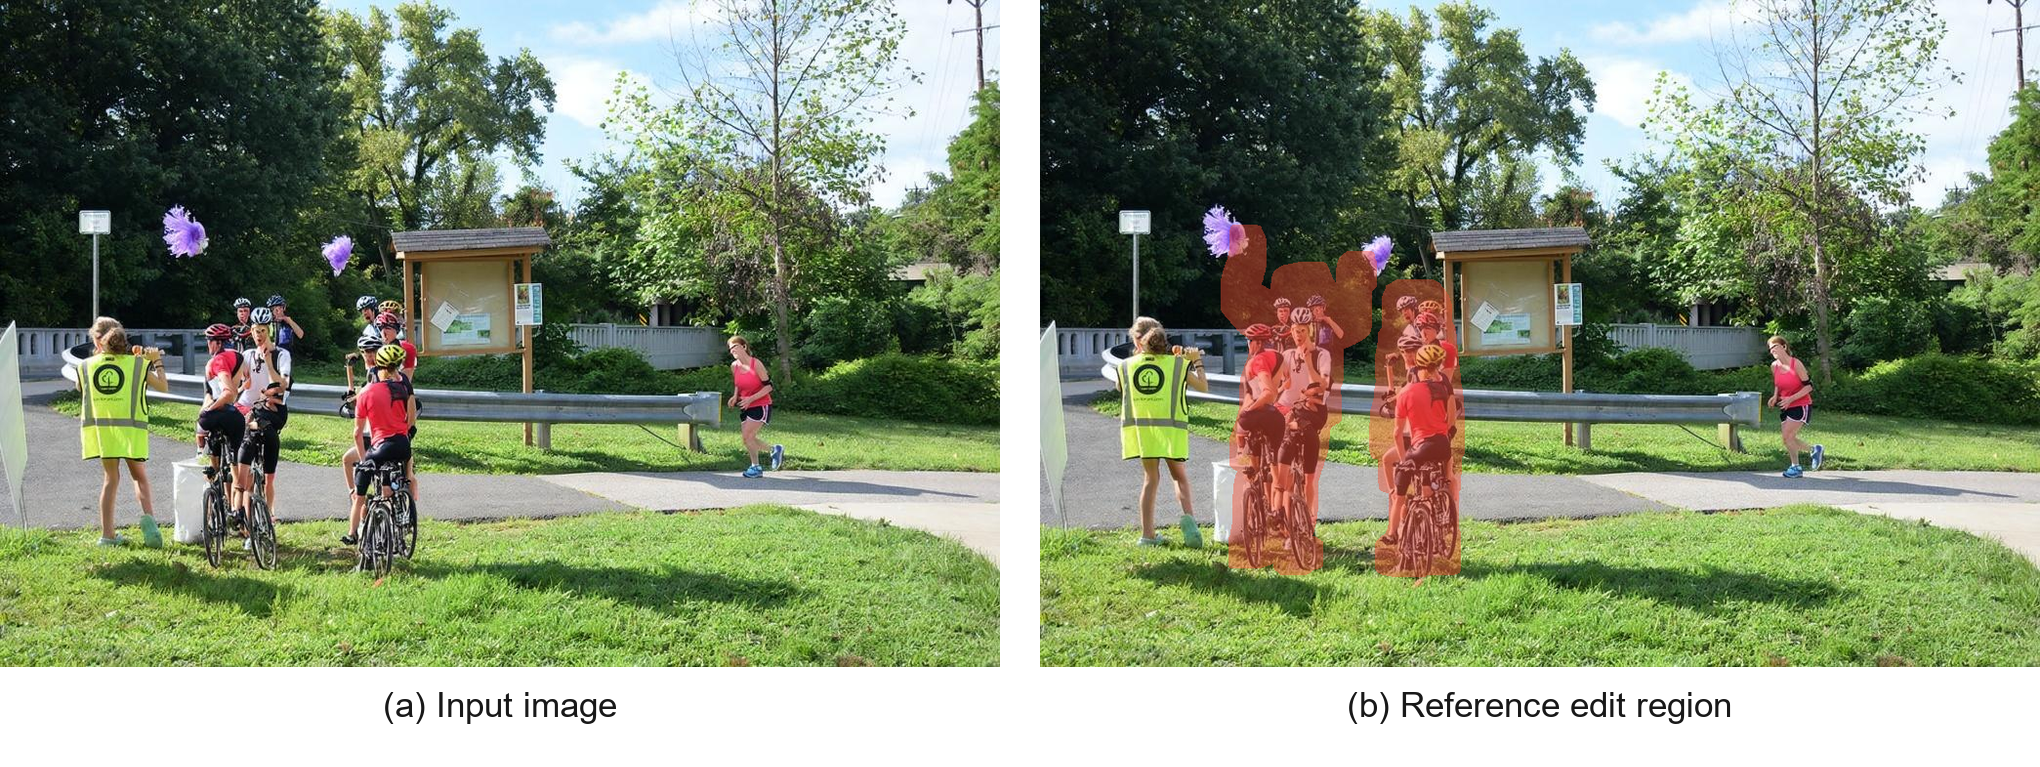
\includegraphics[width=\columnwidth]{figures/introduction_problem.png}
\caption{An inpainted input and its annotated edit region from the development data. The annotation provides a reference for localization evaluation.}
\label{fig:problem}
\end{figure}

Resizing the full image preserves scene context but can smooth cues associated with small edits. Native-resolution tiles retain these details but capture less context. We study whether the same encoder can support both views and whether their scores provide complementary evidence. This design uses one pretrained backbone and requires only a single image at test time.
\clearpage
\section{Related Work}
Image manipulation localization estimates a spatial mask in addition to a global label. TruFor combines visual content and forensic traces~\cite{trufor}. DeCLIP explores how to recover spatial evidence from pretrained CLIP representations~\cite{declip}. OpenSDI introduces OpenSDID and evaluates MaskCLIP across generative settings~\cite{opensdi}. FUSED combines semantic and forensic information using expert routing~\cite{fused}. Our design asks how much can be obtained from a shared ConvNeXt encoder and two task heads when the local path retains the input pixel scale.
\paragraph{Evidence outside the edited area.}
A detector can exploit generator artifacts that extend beyond the annotated region~\cite{inpx}. Consequently, classification accuracy and mask overlap answer different questions. We measure both and inspect genuine-image false alarms in addition to edited-image masks.
\paragraph{Research questions.}
First, does score fusion improve image detection over the same model's whole-image score? Second, does native tiling improve overlap on small edits relative to a resized whole-image mask? Third, how do both measurements change when the image is JPEG recompressed? The proposed experiments hold the source sets constant to isolate each comparison.
\clearpage
\section{Architecture}
We use an ImageNet-pretrained ConvNeXt-Tiny encoder~\cite{convnext}. The whole-image path receives a bilinearly resized $384\times384$ RGB image. The local path receives overlapping $384\times384$ tiles on a grid with 256-pixel stride. The final tile on each axis is anchored at the image edge. Images smaller than a tile are padded, and padding is excluded during reconstruction and loss computation.

\begin{figure}[t]
\centering
\small
\begin{tabular}{c}
\fbox{Single RGB image}\\
$\downarrow$\\
\fbox{Whole-image resize and native tiles}\\
$\downarrow$\\
\fbox{Shared ConvNeXt-Tiny encoder}\\
$\swarrow\qquad\searrow$\\
Whole-image score \quad Tile masks\\
$\quad\searrow\qquad\downarrow$\\
\shortstack{Score fusion $\leftarrow$ Merged probability map\\
$\downarrow$\hspace{6em}$\downarrow$\\
Image decision\hspace{2em}Edit mask}
\end{tabular}
\caption{Whole-image and tile paths share encoder weights. The merged map supplies both the mask and a local classification score.}
\label{fig:architecture}
\end{figure}
Global average pooling of the final encoder stage feeds a linear image classifier. The mask decoder uses lateral projections from the four encoder stages to a common width of 64 channels. A top-down path upsamples and adds adjacent scales, then applies a convolution to produce one logit per location. Bilinear upsampling produces the tile-size output. The two heads operate on different views during deployment.
\clearpage
\section{Training and Inference}
Each training example supplies one whole-image label and a native crop with a matching mask. Edited-image crops include both samples overlapping the edit and uniformly sampled crops. For a crop outside the edit, the reference mask is empty. Spatial flips are applied jointly to a crop and its mask.
\begin{equation}
L=L_{\mathrm{image}}+L_{\mathrm{mask,BCE}}+L_{\mathrm{Dice}}.
\end{equation}
The first term uses binary cross-entropy on the whole-image logit. The pixel BCE uses valid crop pixels and balances foreground and background when both occur. Dice loss is evaluated on crops with an annotated edit. On empty masks, BCE still penalizes false activations.
\paragraph{Reconstruction.}
For pixel $x$, let $p_i(x)$ be the sigmoid output of tile $i$ covering that pixel. The reconstructed map is
\begin{equation}
P(x)=\frac{\sum_{i:x\in i}w_i(x)p_i(x)}
                 {\sum_{i:x\in i}w_i(x)},
\end{equation}
where $w_i$ is a Hann window with a positive floor. The floor retains coverage at the edges. A threshold $\tau_m$ converts $P$ into the binary edit mask.
\paragraph{Image decision.}
Let $s_g$ be the whole-image sigmoid score and $s_l$ the mean of the highest 100 values in $P$, or all values when the image has fewer pixels. The combined score is $s=\alpha s_g+(1-\alpha)s_l$. The image is called edited if $s\geq\tau_d$. Select $\alpha$, $\tau_d$, and $\tau_m$ on validation and freeze them before testing.
\clearpage
\section{Data and Evaluation}
Use the OpenSDID generator groups available in the project~\cite{opensdi}. Group related images by original photograph before forming train, validation, and test splits. Record sample IDs, generator, image label, image dimensions, reference mask, and source group. Verify mask geometry and inspect both classes before training. A test set of 200 images with 100 edited and 100 genuine examples gives a resolution of 0.5 percentage points in ordinary accuracy. If exact balance by generator is feasible, use 20 edited and 20 genuine examples in each of the five groups.
\paragraph{Operating points.}
Select the classification threshold and fusion weight by validation balanced accuracy. Select the mask threshold by validation mean IoU on edited images. Publish the thresholds with the run configuration. Freeze checkpoint selection and inference settings before evaluating the test split.
\paragraph{Metrics.}
Report overall image accuracy, balanced accuracy, edited-class F1, AUROC, and genuine false-positive rate. Compute per-image mask IoU on edited images and average across those images. Report IoU for regions smaller than 2 percent of the image, alongside the number of qualifying samples. Report per-generator figures and the averaging rule. For uncertainty, resample original-image groups and recalculate metrics on the resulting samples.
\paragraph{Target.}
The planned accuracy target is 83.5 percent, equivalent to 167 correct decisions on a 200-image test. Report the observed score, even if it differs from the target.
\clearpage
\section{Comparison Protocol}
Compare checkpoints trained on the same inputs and evaluated on the same held-out source groups when feasible. A published number from a different protocol belongs in a separately identified literature comparison. Hold threshold selection rules, input treatment, and metric aggregation constant for the matched comparison.
\begin{table}[h]
\centering\small
\caption{Planned matched comparison. Every row requires a scored run.}
\begin{tabular}{@{}lp{.56\columnwidth}@{}}
\toprule Method & Role\\\midrule
FRAME & Shared ConvNeXt-Tiny, whole view and tiles\\
FUSED & Semantic and forensic fusion baseline\\
MaskCLIP & OpenSDI detection and localization baseline\\
DeCLIP & Pretrained feature localization baseline\\
\bottomrule
\end{tabular}
\end{table}
\paragraph{Ablations.}
Compare whole-image classification, local pooling alone, and fused scoring on the same predictions. For localization, train the whole-image mask comparison with the same mask loss and comparable training budget. Upsample its predictions to the original dimensions and compare them with the native-tile map. Report tiny-edit IoU and genuine-image false alarms alongside the main metrics.
\paragraph{Runtime.}
Report the device, precision, image dimensions, tile count, and end-to-end latency protocol. Include resize, tile extraction, inference, and reconstruction in latency. Summarize median and 95th-percentile latency across the measured inputs.
\clearpage
\section{Compression and Results Reporting}
Use matched JPEG recompression of genuine and edited test images at quality settings 95, 75, and 50, retaining an as-supplied control. Specify the encoder and chroma subsampling. Keep image dimensions and mask coordinates fixed. Apply the same frozen thresholds at every quality level and report changes in accuracy, genuine false-positive rate, and edited-image IoU.
\begin{table}[h]
\centering\small
\caption{Results table to complete from saved predictions.}
\begin{tabular}{@{}lccc@{}}
\toprule
Input & Acc. & False alarms & Mask IoU\\\midrule
As supplied & Pending & Pending & Pending\\
JPEG 95 & Pending & Pending & Pending\\
JPEG 75 & Pending & Pending & Pending\\
JPEG 50 & Pending & Pending & Pending\\
\bottomrule
\end{tabular}
\end{table}
\paragraph{Qualitative review.}
Show representative inputs, reference masks, probability maps, and thresholded predictions. Include small edits, missed edits, and genuine images with high scores. Select examples by a documented rule. Reference each output to the tested checkpoint and inference settings.
\paragraph{Run artifacts.}
Save the split manifests, checkpoint identifier, training configuration, selected thresholds, image scores, predicted masks, and evaluation script. Compute the table values from these predictions. Check that counts reproduce accuracy and F1 and that averaging per group reproduces the stated aggregate when groups are weighted equally.
\clearpage
\section{Limitations and Conclusion}
A native tile may contain insufficient context to distinguish generation traces from genuine texture. The number of tiles grows with image size, so a single shared encoder reduces model duplication but does not bound per-image inference cost. A fixed top-pixel pool may respond to isolated high scores on textured scenes. Generator and image-source shifts can alter both the score distribution and mask accuracy. JPEG quality tests capture controlled recompression and do not cover arbitrary upload pipelines.
\par
This draft proposes a single-encoder architecture for image classification and edit localization. Whole-image and native-tile views probe complementary evidence with shared ConvNeXt-Tiny weights. The planned evaluation tests the 83.5 percent accuracy target and measures whether local evidence improves classification, small-region overlap, and robustness under recompression.
\clearpage
\bibliographystyle{ACM-Reference-Format}
\bibliography{references}
\end{document}

